\section{The Physics of Nuclear Interactions}

This section provides the physical background needed to understand the probabilities of neutron interactions with matter. Due to the very large neutron densities on the order of \(10^8\) per cm$^3$, neutron interactions with matter will only be regarded in an average sense - for reactor analysis purposes, detailed accounting of every neutron is unneccessary. 

\subsection{Radioactive Decay}
\label{sec:RadioactiveDecay}
Four of the most important types of radioactive decay are:

\begin{enumerate}
\item Alpha decay - a nucleus emits a helium nucleus.
\item Beta decay - in \(\beta^+\) decay, a proton is converted to a neutron plus a positron \(e^+\) and a neutrino. In \(\beta^-\) decay, a neutron is converted to a proton plus an electron \(e^-\) and an antineutrino.
\item Gamma decay - a nucleus transitions from a higher energy state to a lower energy state and in the process emits a photon.
\item Neutron decay - a neutron is emitted.
\end{enumerate}

The physics of radioactive decay are based on the assumption that the probability of decay of a nuclide is constant in time. The probability of decay per unit time, \(\lambda\), is also known as the ``decay constant.'' Given a constant probability for decay, the rate of change of a population depends instantaneously on the size of the population, \(N\), and the probability of decay:

\beq
\label{eq:Decay}
\frac{dN(t)}{dt}=-\lambda N(t)
\eeq

\(\lambda N\) represents the instantaneous number of radioactive decays occurring, and is frequently referred to as the activity, \(A\):

\beq
\label{eq:ActivityDef}
A(t)\equiv\lambda N(t)
\eeq

Activity is typically quoted in units of Curies, or \(3.7\times10^{10}\) decays per second, roughly equivalent to the activity of one gram of radium. Solution of Eq. \eqref{eq:Decay} provides an expression for the number of nuclei present given an initial number \(N_0\):

\beq
\label{eq:DecayEqn}
N(t)=N_0e^{-\lambda t}
\eeq

For systems of multiple nuclides, a system of equations of the form in Eq. \eqref{eq:Decay} exists with additional source terms representing decay chain effects, producing a constant-coefficient linear system. If \(e^{-\lambda t}=1\), no decay occurs, so the probability of no decay occurring between \(0\leq t\leq T\) is equal to \(e^{-\lambda T}\). The cumulative probability of decay in this time interval is obtained as unity minus the probability of no decay:

\beq
\label{eq:DecayCDF}
F(t)=1-e^{-\lambda t}
\eeq

where \(F\) indicates a \gls{cdf}. The expectation value of the lifetime \(\bar{t}\) of a nuclide is calculated by computing the first moment of the instantaneous (i.e. \gls{pdf} of Eq. \eqref{eq:DecayCDF}) probability of decay:

\beqa
\label{eq:MeanLifetime}
\bar{t}\equiv&\int_0^\infty dt\ \lambda e^{-\lambda t}\\
=&\frac{1}{\lambda}
\eeqa

For decay that results in transition in energy levels, such as gamma decay, the Heisenberg uncertainty principle suggests that the energy difference between initial and final states is proportional to the decay constant. It is often the case that very large energy transitions have high decay constants.

\subsection{Nuclear Collisions}
As opposed to radioactive decay discussed in Section \ref{sec:RadioactiveDecay}, the probabilities of nuclear collisions are not constants independent of all environmental factors. For nuclear collisions, the probability of interaction is dependent on both the identities of the two interacting particles and their relative velocity (which accounts for both their relative energy and directions of motion). All nuclear reactions are accompanied by the absorption or release of energy; this energy can be computed based on the mass \(m\) that is converted to energy and vice versa using the following result from general relativity:

\beq
E=mc^2
\eeq

%Additional collisions of importance include \((n,\alpha)\) reactions, common in absorber materials introduced for reactor control. 

The microscopic cross section \(\sigma\) is the fundamental property data required for the analysis of nuclear systems. The microscopic cross section for reaction \(i\), \(\sigma_i\), is {\it proportional} to the probability that a neutron will interact with a specific nucleus through a reaction of type \(i\). More specifically, the microscopic cross section is the probability per nucleus in a target of unit cross-sectional area that a neutron in a beam of intensity \(I\) will interact with it. While not {\it equivalent} to the effective area presented by the target nuclei to a beam, typical units of \(\sigma\) do roughly correspond to the cross sectional area of a nucleus represented as a circle with nuclear radius of \(10^{-12}\) cm. The total cross section is the sum of the scattering and absorption cross sections. While neutrons are released in fission such that it could in some sense be treated as a scattering reaction, fission is customarily treated as an absorption interaction.

The microscopic cross section only indicates the probability of interaction with a single nucleus in a target of unit cross-sectional area. To obtain the probability of interaction per unit distance traveled by the particle, \(\sigma\) must be multiplied by the number density \(N\) of the target material. The macroscopic cross section for reaction \(i\), \(\Sigma_i\), is defined as the probability of interaction per unit travel of a particle with {\it any} nucleus:

\beq
\label{eq:MacroscopicSigmaDef}
\Sigma_i\equiv\sigma_iN
\eeq

Similar to the definition for the cumulative probability of decay in Eq. \eqref{eq:DecayCDF}, but provided that \(\Sigma_t\) is constant in space, which unlike radioactive decay is not necessarily true due to variations in \(N\) and the energy distribution in space, the cumulative probability that a neutron has its first interaction in the spatial interval \(x\) to \(x+dx\) is:

\beq
\label{eq:InteractionCDF}
F(x)=1-\Sigma_te^{-\Sigma_tx}
\eeq

The expectation value of the distance traveled before interacting \(\bar{x}\) is calculated by computing the first moment of the (instantaneous, i.e. \gls{pdf} of Eq. \eqref{eq:InteractionCDF}) probability of interaction:

\beqa
\bar{x}\equiv&\int_0^\infty dx\ x\Sigma_te^{-\Sigma_tx}\\
=&\ \frac{1}{\Sigma _t}
\eeqa

The average distance traveled between interactions, \(\bar{x}\) is commonly referred to as the \gls{mfp}. Multiplication of the macroscopic cross section by the velocity of the particle gives the frequency with which interactions occur. This reaction frequency for interaction type \(i\) in nuclide \(j\) is often referred to as the ``reaction rate frequency:''

\beq
\label{eq:ReactionRateFrequency}
\text{Reaction rate frequency}\equiv \|\vv{v}-\vv{V}\|\sigma_i(\|\vv{v}-\vv{V}\|)N_j
\eeq

where \(\vv{v}\) is the neutron velocity and \(\vv{V}\) the velocity of the target nucleus. Intuitively, the reaction rate and microscopic cross section must be proportional to the relative velocity. Eq. \eqref{eq:ReactionRateFrequency} is written in terms of the particle velocity, rather than the relative velocity, through the use of thermally-average cross sections described in Section \ref{sec:ThermalNeutrons}. By a similar procedure as performed to obtain the average lifetime and path length, the average time between collisions can be calculated as \(1/(v\Sigma)\).\

For all reaction types except potential scattering, described in Section \ref{sec:PotentialScattering}, the incident neutron interacts with the nuclear potential of the target nuclide to form a compound nucleus. A compound nucleus is believed to exist due to the relatively long times observed between interaction with a neutron and subsequent release of reaction products. During this lifetime of the compound nucleus, energy is transferred from the neutron to the nucleons, which after some time leads to the collapse of the compound nucleus. The relatively long lifetime of the compound nucleus makes it very likely that the reaction products are independent of the initial state of the neutron, and only dependent on the state of the compound nucleus. 

The formation of a compound nucleus is a type of resonance reaction; the total energy available to be transferred to the compound nucleus is the sum of the energy in the \gls{cm} frame and the additional binding energy of the neutron. When this total energy closely matches an energy state of the compound nucleus, formation is much more likely to occur, leading to resonance structures in cross sections for reactions involving compound nucleus formation. Because the formation of the compound nucleus leads to some degree of independence of the reaction products on the initial state of the neutron, the energy dependence of the cross sections for many different reactions share common features. 

The neutron wavelength \(\lambda_n\) is proportional to \(1/\sqrt{E}\):

\beq
\label{eq:NeutronWavelength}
\lambda_n=\frac{h}{\sqrt{2mE}}
\eeq

where \(h\) is the Planck constant and \(\sqrt{2mE}\) is the momentum of the neutron. There are generally four regions of unique behavior in the total scattering cross section for {\it light} nuclei, bounded by the approximate energy ranges:

\begin{itemize}
\item \(10^{-4}-10^{-2}\) eV - the neutron wavelength becomes on the order of the spacing between atoms such that a neutron interacts with groups of nuclei simultaneously, and thermal motion of the target cannot be neglected. If the target material is organized in a lattice, the neutron is diffracted, and a sensitive energy dependence exists as the neutron energy approaches multiples of the interatomic spacing between different ``views'' of the lattice. Thresholds for this type of interaction typically occur at \(10^{-3}\) eV and above. The neutron may excite lattice vibrations or rotate atoms. 
\item \(10^{-2}-10^{+6}\) eV - the scattering cross section is dominated by potential scattering; because \(\sigma_p\) is approximately independent of energy, this gives a nearly constant \(\sigma_s\) 
\item \(10^{+6}-10^{+7}\) eV - resonance region; large peaks are observed where \(E_c+E_b\) coincides with an excited state of the compound nucleus
\item Above \(10^{+7}\) eV - fast spectrum region; high energies result in very small wavelengths, making interaction improbable.
\end{itemize}

Heavy nuclei have overlapping resonances that begin in the eV to keV, range, while light nuclei, if resonances are present at all, have resolved resonances in the MeV range. The overlapping resonance region in heavy nuclei is referred to as the \gls{urr}, as experimental measurements cannot resolve the resonances. Both light and heavy nuclei are characterized by inelastic scattering at very high energies. Intermediate energies are dominated by potential scattering for light nuclei and radiative capture and elastic scattering for heavy nuclei. 

Cross section data, especially for resonances, tends to be stored as a function of several fitting parameters rather than cross sections tabulated at discrete energies in order to reduce the required storage. Processing codes such as NJOY then convert the cross section data to a useable form for computational activities. 

\subsubsection{Radiative Capture}

The radiative capture cross section \(\sigma_\gamma\) exhibits strong resonance structure, since absorption of a neutron leads to the formation of a compound nucleus that decays by transitioning between different energy states through the release of a cascade of photons. Radiative capture is an important interaction due to its removal of neutrons from the fission chain reaction. As temperatures increase, radiative capture resonances broaden, resulting in increased radiative capture reaction rates in nuclides such as U-238, which in most reactor designs leads to negative reactivity feedback. Radiative capture is also the primary mechanism by which U-238 is transmuted to Pu-239.

U-238 has several low-lying resonances in the eV range, with the lowest resonance at 6.67 eV with a narrow width of 0.027 eV and a peak of \(7\times10^3\) barns that is about four orders of magnitude larger than the nearby cross section. Radiative capture cross sections tend to be largest at low energies, and generally decrease continuously with energy except for the presence of resonances. For low energies, \(\sigma_\gamma\propto1/v\), while at higher energies falls off very quickly with energy as \(\sigma_\gamma\propto1/\sqrt{E^5}\).

\begin{comment}
For resonances that are widely separated from one another, the energy dependence of \(\sigma_\gamma\) can be approximated using the Breit-Wigner single-level resonance formula:

\beq
\label{eq:BW}
\sigma_\gamma(E_c)=\sigma_0\frac{\Gamma_\gamma}{\Gamma}\sqrt{\frac{E_0}{E_c}}\left\lbrack1+4\left(\frac{E_c-E_0}{\Gamma}\right)^2\right\rbrack^{-1}
\eeq

where \(E_0\) is the energy on which the resonance is centered; \(\Gamma\) is the total line width of the resonance, which captures the width of the energy level at the \gls{fwhm}; and \(\Gamma_\gamma\) is the radiative line width, which captures the probability that the compound nucleus decays via the emission of a photon. \(\sigma_0\) is the total cross section at \(E_0\) which scales as:

\beq
\sigma_0\propto\frac{(A+1)^2}{A^2E_0}\sqrt{E}
\eeq

but also depends on other factors such as spin. Because resonance effects are most significant in heavy nuclei, \(E_c\) is well-approximated by \(E\). 
\end{comment}

Radiative capture in U-238 and Th-232 produce fissile isotopes through the following decay chains:

\begin{equation*}
\text{U-238} + n\rightarrow \text{U-239}\rightarrow \text{Np-239}\rightarrow \text{Pu-239}
\end{equation*}

\begin{equation*}
\text{Th-232}+n\rightarrow \text{Th-233}\rightarrow \text{Pa-233}\rightarrow \text{U-233}
\end{equation*}

In order to ``breed'' more fissile material than consumed, the number of neutrons produced per neutron absorbed, \(\eta\), must exceed unity:

\beqa
\label{eq:Eta2Def}
\eta\equiv&\frac{\text{average number of neutrons produced}}{\text{average number of neutrons absorbed}}\\
=&\frac{\sum_{i=1}^N\nu_i\Sigma_{f,i}}{\sum_{i=1}^N\Sigma_{a,i}}
\eeqa

where \(N\) is the total number of types of fissile isotopes present in the fuel mixture. \(\eta\) is slightly greater than two in the thermal and epithermal range, but dramatically increases above 10 keV, indicating the onset of an energy range in which breeding is more easily achievable. In the fast energy range, \(\eta\) is largest for Pu-239 and Pu-241. Breeding in a thermal spectrum is only possible for U-233, for which \(\eta\approx2.4\). 

\subsubsection{Fission Reactions}

Fission is the splitting of a heavy nucleus into lighter fragments, releasing energy. Energy is released for fission of heavy nuclides because the maximum binding energy per nucleon of 8.7 MeV is observed at \(A=50\); the binding energy per nucleon decreases for heavier nuclides, so fissioning to produce lighter nuclei increases the binding energy per nucleon of the products. Spontaneous fission is relatively uncommon, despite the possibility of greatly increasing the stability of the product nuclides, because a 6-9 MeV fission barrier height exists for most heavy nuclei. This barrier height can be overcome with either the binding energy of a neutron (plus its kinetic energy) or the kinetic energy of a different particle such as a gamma ray. Such photon-induced fission is known as ``photofission.'' Spontaneous fission occurs through the barrier penetration mechanism of quantum mechanics, and hence is characterized by relatively low probabilities. 

Nuclei with fission barriers that can be exceeded by neutrons of low energy are termed ``fissile,'' while heavy nuclei with slightly higher fission barriers that require high-energy neutrons to fission are termed ``fissionable.'' Fissionable nuclei cannot sustain a fission chain reaction on their own, and fast reactor designs must always include some fissile nuclides to sustain the chain reaction. % why?

Because fission is a compound nucleus process, the fission cross section is characterized by resonance structures. For fissile nuclides, the fission cross section is on the order of several hundred barns in the thermal range, about two orders of magnitude higher than in the fast neutron range. For fissionable nuclides, the fission cross section tends to display a threshold energy below which the cross section is essentially zero due to insufficient energy needed to exceed the fission barrier. However, the fission cross section above this threshold tends to be rather small, on the order of several barns, similar to the high-energy behavior in fissile nuclides. The fast fission cross section is larger for Pu-242 and Pu-240, and much lower for Th-232 and U-238. 

Over almost all ranges in energy, the fission cross section is greater than the capture cross section. At low energies, fission is approximately five times more likely than capture in U-235; at low energies, the ratio of fission to capture is highest for U-235, making it in this sense the ``best'' fuel for thermal systems. At high energies, the capture cross section decreases much more rapidly than the fission cross section, indicating that the fission process is more ``efficient'' at high energies. However, due to the much lower cross sections involved, this lower rate of absorption must be compensated by much higher fuel densities to obtain the same fission reaction rates. 

The goal of most nuclear reactor designs is to fission the nuclides within the core, but some reactors are also designed with the goal of transmuting significant quantities of non-fissile isotopes to fissile isotopes in a process known as ``conversion.'' This process is referred to as ``breeding'' if \(\eta\) is significantly larger than two to permit one fertile capture per fission. Neutron capture by fertile isotopes produces fissile isotopes with an efficiency defined as the conversion ratio:

\beq
\label{eq:ConversionRatioDef}
\text{conversion ratio}\equiv\frac{\text{rate of fissile atom production}}{\text{rate of fissile atom destruction}}
\eeq

Conversion ratios in \glspl{lwr} typically range in the 0.5 to 0.7 range due to transmutation of U-238 to Pu-239. A typical fast reactor design has a breeding ratio on the order of 1.2.

Each fission produces fission products, neutrons, photons, beta particles, and neutrinos. As nuclides become heavier, it becomes more probable to have a greater number of neutrons than protons to reduce the repulsive effects in a very large nucleus. Therefore, after fission, each fission product tends to be rather neutron rich for its mass number, and tends to undergo \(\beta^-\) decay. Approximately 80\% of the total fission energy release is manifested in the kinetic energy of fission fragments, which move on average only about 0.1 mm from the site of fission. The remaining 20\% of the energy is approximately evenly-distributed amongst neutrons, gamma energy, beta decay of fission products, neutrinos, and non-fission reactions due to neutron capture in non-fissionable materials. The gamma ray energy (in motion and capture) tends to be deposited up to about 1 m away from the site of fission, thus coupling relatively distant regions of the reactor.

The neutrons born nearly instantaneously following fission from the fragmentation of the compound nucleus are considered ``prompt'' neutrons. Delayed by up to several hundred seconds is another source of neutrons from the decay of fission products. Rather than consider the build up and decay of fission products with the Batemann equations on time scales of seconds to capture this delayed source of neutrons, these ``delayed'' neutrons are treated as a time-lagged fission source of neutrons. While it is not possible to change the source of prompt neutrons by removing compound nuclei from the control volume before decay (such time scales are much smaller than nanoseconds), it is possible to remove the fission products whose decay produces neutrons. Distinguishing between these two types of neutrons permits flexibility in transient analysis of nuclear systems. The average total number of neutrons born in fission from an incident neutron at energy \(E\), \(\nu(E)\), tends to increase linearly with incident neutron energy. For U-235, \(\nu\) can be approximated as:
% does beta remain constant in energy, or does this statement simply indicate that the number of prompt neutrons increases with energy?
\beq
\label{eq:U235_nu}
\nu(E)=\begin{cases}2.432+0.066\times10^{-6}E & E\leq 10^6\text{ eV}\\
2.349 + 0.15\times10^{-6}E & E>10^6\text{ eV}
\end{cases}
\eeq

For Pu-239, \(\nu\) can be approximated as:

\beq
\label{eq:Pu239_nu}
\nu(E)=2.874+0.138\times10^{-6}E
\eeq

where \(E\) is given in eV in Eqs. \eqref{eq:U235_nu} and \eqref{eq:Pu239_nu}. For thermal fission in U-235 and Pu-239, \(\nu\) is approximately 2.43 and 2.87, respectively. 

The energy and angle spectrum of the fission neutrons depends on the fissioning nuclide and incident neutron energy, though to a lesser degree on the incident neutron energy than \(\nu\). These spectrums differ for prompt and delayed neutrons, but both have very weak angular dependence such that isotropy is commonly assumed. The prompt fission neutron energy spectrum for U-235 with angular dependence integrated out can be approximated as:

\beq
\label{eq:U235_prompt}
\chi_p(E)=0.453e^{-1.036\times10^{-6}E}\sinh{(\sqrt{2.29\times10^{-6}E})}
\eeq

where \(E\) is given in eV. The average prompt fission neutron energy predicted by Eq. \eqref{eq:U235_prompt} for U-235 is 1.98 MeV, while the most probable fission neutron energy is 0.72 MeV. The prompt fission neutron spectrum for Pu-239 with angular dependence integrated out can be approximated as:

\beq
\label{eq:Pu239_prompt}
\chi_p(E)=0.6739\sqrt{E\times10^{-6}}e^{-E/1.41}
\eeq

where \(E\) is given in eV. The average prompt fission neutron energy predicted by Eq. \eqref{eq:Pu239_prompt} for Pu-239 is 2.12 MeV, while the most probable fission neutron energy is 0.71 MeV. U-235 therefore has a slightly lower-energy prompt fission neutron energy spectrum than Pu-239. While Eqs. \eqref{eq:U235_prompt} and \eqref{eq:Pu239_prompt} represent closed-form (approximate) prompt fission neutron energy distributions, the fission spectrum information is most frequently utilized in tabular form available with cross section data.

The fraction of neutrons born delayed, \(\beta\), is defined as the sum of the fraction of neutrons produced from delayed decay of fission products in \(J\) delayed neutron precursor groups,

In order to separate the total fission source into a prompt and delayed term for transient analyses, the fraction of neutrons born delayed is defined as \(\beta\):

\beq
\label{eq:BetaDef}
\beta\equiv\ \sum_{j=1}^J\beta_j
\eeq

Approximately 45 different nuclides produced in the decay chain of the fission products decay by neutron decay, but \(J\) is typically approximated as a smaller number by grouping the precursors according to their half-lives for neutron decay. These half-lives are the half-lives characterizing the time to emit a neutron via neutron decay from the time of fission, and therefore include any intermediate decays that do not produce neutrons. The longest of these half-lives is approximately 55 seconds corresponding to Br-87. While \(\beta\) is a function of energy, the relationship is fairly weak below 4 MeV and is commonly neglected. Table \ref{table:beta} shows \(\beta\) for thermal and fast fission of various isotopes.

\begin{table}[H] 
\caption{\(\beta\) for common nuclides of interest.}
\centering
\begin{tabular}{c c c}
\hline\hline
Nuclide & Fission Energy & \(\beta\)\\
\hline
Th-232 & fast & 0.02270\\
U-238 & fast  & 0.01560\\
Pu-239 & fast & 0.00206\\
Pu-241 & fast & 0.00530 \\
U-235 & thermal & 0.00644 \\
U-233 & thermal & 0.00264 \\
\hline
\end{tabular}
\label{table:beta}
\end{table}

The delayed neutron group structure is dependent on the fissioning isotope, but relatively independent of the incident neutron energy, and hence these group structures can be used for both fast and thermal systems. The group structure for U-235 is shown in Table \ref{table:U235_delayed}.

\begin{table}[H]
\caption{Six-group delayed neutron precursor structure for U-235.}
\centering
\begin{tabular}{c c c}
\hline\hline
Group & Half-Life (s) & \(\beta_j/\beta\)\\ [0.5ex]
\hline
1 & 54.51 & 0.038 \(\pm\) 0.004\\
2 & 21.84 & 0.213 \(\pm\) 0.007\\
3 & 6.00 & 0.188 \(\pm\) 0.024\\
4 & 2.23 & 0.407 \(\pm\) 0.010\\
5 & 0.496 & 0.128 \(\pm\) 0.012\\
6 & 0.179 & 0.026 \(\pm\) 0.004\\
\hline
\end{tabular}
\label{table:U235_delayed}
\end{table}

The energy spectrum of the \(j\)-th group of delayed neutrons, \(\chi_{d,j}(E,\hO)\), is significantly lower than the energy spectrum of prompt neutrons. Typical delayed neutron energies are on the order of 0.5 MeV, rather than 2 MeV for prompt neutrons. While Eqs. \eqref{eq:U235_prompt} and \eqref{eq:Pu239_prompt} depict relatively smoothly-varying energy spectrums, the energy spectrum for delayed neutrons is not such a smooth distribution, and varies significantly with the group.

Additional sources of delayed neutrons aside from fission product neutron decay include photoneutron interactions, which may be a significant source of neutrons in systems with deuterium and beryllium. These photoneutron reactions typically have very long half-lives, on the order of two hours, and can be approximated through the use of additional delayed neutron groups.

\subsubsection{Potential Scattering Reactions}
\label{sec:PotentialStationary}

In a potential scattering reaction, two colliding bodies interact as hard spheres without forming a compound nucleus. There is very weak energy dependence in potential scattering, and the cross section is often well-approximated by the cross-sectional area of the target nuclide nucleus for intermediate energies. The radius of a nucleus for a nuclide with mass number \(A\) can be approximated as:

\beq
R\ (\text{cm})\approx1.25\times10^{-13}A^{1/3}
\eeq

For U-235, \(\sigma_p\approx7.5\) barns. The energy and angle dependence of the double differential potential scattering cross section can be determined analytically using conservation of momentum and energy for scattering from stationary low-\(A\) nuclides for neutron energies less than 1 MeV. The potential scattering cross section can be decomposed into a probability of interaction at energy \(E\) multiplied by the probably of an incoming energy and angle \(E\) and \(\hO\) being scattered to an outgoing energy and angle \(E'\) and \(\hO\):

\beq
\label{eq:DifferentialSigma}
\sigma_p(E\rightarrow E',\hO\rightarrow\hO')=\sigma_p(E)P(E'\rightarrow E)P(\hO\rightarrow\hO')
\eeq

For potential scattering off stationary nuclei, these two probabilities can be calculated as follows. It will be useful to transform the coordinate system to the \gls{cm} frame. The velocity of the center of mass frame \(\vv{\mathscr{V}}\) is calculated as the mass-weighted velocities in the lab frame:

\beq
\label{eq:CMVelocity}
\vv{\mathscr{V}}\equiv\frac{m\vv{v}+M\cancel{\vv{V}}}{m+M}
\eeq

where \(m\) is the neutron mass and \(M\) the target nuclide mass. Quantities without a \(CM\) subscript represent the lab-frame quantities. In this analysis, it is assumed that the target nucleus is stationary in the lab frame such that \(\vv{V}=0\). The velocities in the \gls{cm} frame of the neutron and target nucleus are:

\beqa
\label{eq:CMVelocities}
\vv{v}_{CM}=&\vv{v}-\vv{\mathscr{V}}\\
=&\frac{M/m}{1+M/m}\vv{v}
\eeqa

\beqa
\label{eq:CMVelocities2}
\vv{V}_{CM}=&\cancel{\vv{V}}-\vv{\mathscr{V}}\\
=&\frac{1}{1+M/m}\vv{v}
\eeqa

where Eq. \eqref{eq:CMVelocity} was used for \(\vv{\mathscr{V}}\). The total momentum in the \gls{cm} frame is obtained by multiplying masses with the velocities in the \gls{cm} frame in Eqs. \eqref{eq:CMVelocities} and \eqref{eq:CMVelocities2} and summing, which shows that the total momentum in the \gls{cm} frame is zero (which is also the {\it definition} of the \gls{cm} frame). The kinetic energies in the lab and \gls{cm} frame are:

\beq
\label{eq:ELab}
E=\frac{1}{2}\left(m\|\vv{v}\|^2+M\cancel{\|\vv{V}\|^2}\right)
\eeq

\beqa
\label{eq:ECM}
E_{CM}=&\ \frac{1}{2}\left(m\|\vv{v}_{CM}\|^2+M\|\vv{V}_{CM}\|^2\right)\\
=&\ \frac{1}{2}\frac{Mm}{M+m}\|\vv{v}\|^2
\eeqa

The energies in the lab and \gls{cm} are related through Eqs. \eqref{eq:ELab} and \eqref{eq:ECM} as:

\beq
E_{CM}=\frac{M}{M+m}E
\eeq

from which it can be seen that the energy in the \gls{cm} is always less than the energy in the lab frame because some energy is allocated to the movement of the \gls{cm} frame itself via \(\vv{\mathscr{V}}\). Using conservation of momentum and energy, it can be shown that the velocity magnitudes of the projectile and target following the collision in the \gls{cm} frame remain constant - only the velocity vectors are rotated through an angle \(\theta_c\) in the \gls{cm} frame. Rearranging Eq. \eqref{eq:CMVelocities} and defining \(\theta\) as the lab frame scattering angle, two relationships can be written:
% derivation showing that velocity magnitudes remain constant in CM frame pre- and post-collision is missing

\begin{subequations}
\label{eq:CMvsLab}
\begin{eqnarray}
v'\sin{(\theta)}&=&v'_{CM}\sin{(\theta_c)}\\
v'\cos{(\theta)}&=&v'_{CM}\cos{(\theta_c)}+\mathscr{V}
\end{eqnarray}
\end{subequations}


\begin{tcolorbox}[breakable]
Dividing Eq. \eqref{eq:CMvsLab}a by Eq. \eqref{eq:CMvsLab}b gives the relationship between the lab and \gls{cm} frame scattering angles:

\beq
\label{eq:CMtoLab}
\tan{(\theta)}=\frac{\sin{(\theta_c)}}{m/M+\cos{(\theta_c)}}
\eeq

Cross sections are typically measured in the \gls{cm} and utilized computationally in the lab frame, so Eq. \eqref{eq:CMtoLab} is useful for transforming measured angular-dependent cross sections to the lab frame. Eq. \eqref{eq:CMtoLab} only represents a transformation of the scattering angles - to transform the angular differential cross sections, write such cross sections in differential form using the \(\theta\) component of the solid angle differential in Eq. \eqref{eq:DifferentialOmega}:

\beq
\sigma\sin{(\theta)}d\theta=\sigma_{CM}\sin{(\theta_{CM})}d\theta_{CM}
\eeq

which gives the following relationship between the lab and \gls{cm} angular differential cross sections:

\beq
\sigma(\theta)=\sigma_{CM}(\theta_{CM})\frac{\left\lbrack\frac{m^2}{M^2}+\frac{2m}{M}\cos{(\theta_{CM})}+1\right\rbrack^{3/2}}{1+\frac{m}{M}\cos{(\theta_{CM})}}
\eeq
% derivation missing
\end{tcolorbox}

Applying the law of cosines between the triangle formed by \(\vv{v}_{CM}'\), \(\vv{v}'\), and \(\vv{\mathscr{V}}\) gives:

\beqa
\label{eq:FinalVelocity}
(v')^2=&\ (v'_{CM})^2+\mathscr{V}^2-2v'_{CM}\mathscr{V}\cos{(\pi-\theta_{CM})}\\
=&\ \frac{M^2/m^2+1+2M/m\cos{(\theta_{CM})}}{(1+M/m)^2}v^2\\
\eeqa

where Eqs. \eqref{eq:CMVelocities} and \eqref{eq:CMVelocities2} have been used along with the identity \(\cos{(\pi-x)}\equiv-\cos{(x)}\). Because kinetic energy is proportional to \(v^2\), and masses do not change during an elastic scattering collision, Eq. \eqref{eq:FinalVelocity} can equivalently be written in terms of the initial and final energies:

\beqa
\label{eq:ElasticScatE}
\frac{E'}{E}=&\ \frac{M^2/m^2+1+2M/m\cos{(\theta_{CM})}}{(1+M/m)^2}\\
=&\ \frac{1}{2}\left\lbrack(1+\alpha)+(1-\alpha)\cos{(\theta_{CM})}\right\rbrack\\
\eeqa

where \(\alpha\) is defined as:

\beq
\alpha\equiv\left(\frac{M/m-1}{M/m+1}\right)^2
\eeq

Eq. \eqref{eq:ElasticScatE} shows that there is a one-to-one relationship between the energy transfer in elastic scattering off stationary nuclei and the \gls{cm} scattering angle. Eq. \eqref{eq:ElasticScatE} also shows that, for a given value of \(\alpha\), \(\theta_{CM}=0\) corresponds to the minimum energy loss (a ``miss'') and \(\theta_{CM}=\pi\) to the maximum energy loss (backscattering). For a given value of \(\alpha\), the maximum energy loss in a single collision therefore corresponds to backscattering, for which Eq. \eqref{eq:ElasticScatE} gives \(E'=\alpha E\). Therefore, to lose the maximum amount of energy, \((1-\alpha)E\), in a single collision, \(\alpha\) should be small, which occurs for small \(M/m\), or very light nuclei. Table \ref{table:FractionalEnergyLoss} shows the maximum fractional energy loss normalized by \(E\) for elastic scattering off stationary nuclei, where \(M/m\) is approximated as \(A\); as can be seen, lighter nuclides are dramatically more effective thermalizers.

\begin{table}[H]
\caption{Maximum fractional energy loss normalized by \(E\) for elastic scattering off stationary nuclei for several common nuclei.}
\centering
\begin{tabular}{c c c}
\hline\hline
Nuclide & \(\alpha\) & Fractional Energy Loss\\ [0.5ex]
\hline
H-1 & 0.00 & 1.00\\
H-2 & 0.11 & 0.89\\
C-12 & 0.72 & 0.28\\
U-235 & 0.98 & 0.02\\
\hline
\end{tabular}
\label{table:FractionalEnergyLoss}
\end{table}

Because there is a one-to-one relationship between the energy loss and scattering angle in the \gls{cm} frame, we can postulate that there is similarly a one-to-one relationship between \(P(E\rightarrow E')\) and \(P(\hO_{CM}\rightarrow\hO_{CM}')\). The probability of scattering from \(\hO_{CM}\) to \(\hO'_{CM}\) multiplied by the total scattering cross section, is simply equal to the differential scattering cross section according to Eq. \eqref{eq:DifferentialSigma}:

\beq
\sigma_sP(\hO_{CM}\rightarrow\hO'_{CM})d\hO'_{CM}=\sigma_{CM}(\theta_{CM})2\pi\sin{(\theta_{CM})}d\theta_{CM}
\eeq

where the scattering is assumed azimuthally symmetric such that \(\sigma_{CM}\) can be written as a function of a single scattering angle \(\theta_{CM}\). Assuming this one-to-one relationship gives:

\beq
\label{eq:OnetoOneEHO}
P(E\rightarrow E')dE'=-\frac{\sigma_{CM}(\theta_{CM})}{\sigma_s}2\pi\sin{(\theta_{CM})}d\theta_{CM}\\
\eeq
% don't know why the RHS is negative

Differentiating Eq. \eqref{eq:ElasticScatE} to obtain \(dE'\) and plugging into \eqref{eq:OnetoOneEHO} gives the differential energy component of the elastic scattering cross section:

\beq
\label{eq:ScatteringDifferentialProb}
P(E\rightarrow E')=\begin{cases}\frac{4\pi\sigma_{CM}(\theta_{CM})}{(1-\alpha)E\sigma_s} & \alpha E\leq E'\leq E\\
0 & \text{else}
\end{cases}
\eeq

For light nuclei and energies less than about 10 MeV, \(\sigma_{CM}\) is isotropic such that:

\beq
\label{eq:IsotropicSigmaCM}
\dhOprime\sigma_{CM}(\hO\rightarrow\hO')=\frac{\sigma_s}{4\pi}
\eeq

Isotropic scattering in the \gls{cm} frame is known as s-wave scattering, and is the most common type of elastic scattering in nuclear reactor applications. For heavier nuclides, a slight angular dependence exists in \(\sigma_{CM}\); however, because the most significant energy losses via elastic scattering occur via scattering off light nuclei, it is a reasonable approximation for {\it all} nuclei to assume isotropic elastic scattering in the \gls{cm} frame. Inserting Eq. \eqref{eq:IsotropicSigmaCM} into Eq. \eqref{eq:ScatteringDifferentialProb} gives the energy differential portion of the s-wave elastic scattering differential cross section:

\beq
\label{eq:SWaveScattering}
P(E\rightarrow E')=\begin{cases}\frac{1}{(1-\alpha)E} & \alpha E\leq E'\leq E\\
0 & \text{else}
\end{cases}
\eeq

Eq. \eqref{eq:SWaveScattering} shows that the probability of scattering to a final energy \(E'\) is independent of this energy, and the final energy probability distribution is uniformly distributed because the elastic scattering angle is also uniformly distributed when isotropy is assumed. Using Eq. \eqref{eq:SWaveScattering}, the average outcoming energy in an elastic scattering collision of a stationary nucleus with an isotropic \gls{cm} scattering cross section is calculated as:

\beqa
\bar{E'}\equiv&\int_{\alpha E}^E dE' E'P(E\rightarrow E')\\
=&\frac{1}{2}E(1+\alpha)
\eeqa

Therefore, the average energy loss is the average of the maximum and minimum energy losses, an intuitive result based on the assumption of isotropy and a one-to-one relationship between scattering angle and energy loss, which resulted in the probability of scattering to \(E'\) being uniformly distributed in the range \(\alpha E\leq E'\leq E\).

\subsubsection{Elastic Resonance Scattering Reactions}

In an elastic scattering reaction, no energy is transferred to the target, so the sum of the initial and final energies is the same. The compound nucleus disintegrates into a neutron and the same target nuclide in its initial energy state. While a resonance structure is present, the behavior is different from resonances observed in the radiative capture and fission cross sections - the cross section may decrease in the vicinity of a resonance because elastic resonance scattering may interfere in a quantum mechanical mechanism with potential scattering.

\subsubsection{Inelastic Scattering Reactions}

In an inelastic scattering reaction, a compound nucleus forms whose disintegration produces a neutron and a product nuclide in an excited state. Inelastic scattering is in a sense equivalent to radiative capture, but with emission of a neutron instead of a photon. Inelastic scattering is only significant at relatively high energies on the order of 10 keV, but is an important mechanism in neutron slowing down in fast systems where potential scattering results in less energy loss per collision than in scattering off light nuclei. In fact, \glspl{lwr} typically have a larger {\it very} fast flux than fast systems due to the lack of heavy nuclei such as sodium from which inelastic scattering is significant. Effective neutron shields can be designed of a layer of high inelastic scattering material (high-\(A\)) which slows neutrons to the epithermal range, after which a low-\(A\) material can be used to effectively reduce energy through potential and elastic scattering. 

An energy threshold typically exists below which inelastic scattering does not occur because the sum of the energy in the \gls{cm} frame and the neutron binding energy is too low to leave the product nucleus in an excited state while producing a neutron with non-zero energy. Heavy nuclei tend to have low-lying excited states, so inelastic scattering becomes probable for heavy nuclei at lower energies than would be possible for lighter nuclei. 

\subsection{The Effects of Relative Motion}
\label{sec:ThermalEffects}

Unless the material is at 0 K, the target nuclide will always have nonzero motion, which cannot be neglected for slow neutrons and cross section resonances characterized by extremely sensitive dependence to the relative energy. In addition, at sufficiently low energies, relative motion must be considered to account for upscattering. The remainder of this section discusses these three effects.

\subsubsection{Thermal Neutrons}
\label{sec:ThermalNeutrons}

The target nuclide velocity \(\vv{V}\) in Eq. \eqref{eq:ReactionRateFrequency} is not identical for each nuclide in the target material because thermal motions occur randomly. However, in a laboratory setting, when measuring microscopic cross sections it is impossible to measure the velocity of each target nucleus to compute the relative velocity. Therefore, some averaging approach is required to account for the relative motion such that quantities in the \gls{nte} can be computed only as a function of the neutron velocity, a tracked quantity. Assume the probability distribution characterizing the distribution in \(\vv{V}\) is given as \(\mathscr{M}\). Define a cross section averaged over the thermal motion of the target nuclei as:

\beq
\label{eq:OneOverV}
\bar{\sigma}v\equiv\int d\vv{V}\sigma\left(\left\Vert\vv{v}-\vv{V}\right\Vert\right)\left\Vert\vv{v}-\vv{V}\right\Vert\mathscr{M}(\vv{V})
\eeq

where this averaged cross section is defined such that the reaction rate frequency in Eq. \eqref{eq:ReactionRateFrequency} can be written proportional to \(v\) rather than the relative velocity. In writing the \gls{nte} and all secondary forms, cross sections are implied to correspond to target-velocity-weighted cross sections \(\bar{\sigma}\) through application of broadening routines. For nuclei that can be well-approximated as an ideal gas in thermal equilibrium, \(\mathscr{M}\) can be replaced by the Maxwell-Boltzmann distribution described in Section \ref{sec:MB}.

At thermal energies, the cross section is inversely proportional to the relative velocity such that \(\sigma(\|\vv{v}-\vv{V}\|)=C/\|\vv{v}-\vv{V}\|\) for some constant \(C\); for this case, Eq. \eqref{eq:OneOverV} becomes:

\beqa
\label{eq:ThermalNeutronProp}
\bar{\sigma}=&\ \frac{C}{v}\int d\vv{V}\mathscr{M}(\vv{V})\\
=&\ \frac{C}{v}
\eeqa

Provided the cross section is inversely proportional to the relative speed, the thermally-averaged cross section is {\it also} inversely proportional to the neutron speed, as expected. The expected inverse velocity proportionality at low energies can be elucidated from Eq. \eqref{eq:OneOverV} by assuming \(\vv{v}\ll\vv{V}\):

\beq
\label{eq:OneOverV2}
\bar{\sigma}v=\int d\vv{V}\sigma(V)VM(\vv{V})
\eeq

The \gls{rhs} of Eq. \eqref{eq:OneOverV2} is a constant independent of \(v\), which demonstrates the inverse-velocity proportionality of \(\bar{\sigma}\). At very low neutron speeds, the probability of interaction becomes dependent solely on the velocity distribution of the target nuclei, and hence the collision frequency \(v\bar{\sigma}N\) ceases to depend at all on the velocity distribution of the neutrons and only on the velocity distribution of the target nuclei. 

\subsubsection{The Doppler Effect}

At all neutron energies, thermal motion must be considered if the cross section is extremely rapidly-varying in energy. Changes in temperature change the velocity distribution of the target nuclei; increases in temperature result in broader ranges in energy of the target nuclei, which results in broadening of cross sections, an effect known as ``Doppler'' broadening. This Doppler effect can be accounted for by integrating the cross section energy dependence over a resonance with an appropriate target nuclide velocity distribution \(\mathscr{M}\) using Eq. \eqref{eq:OneOverV} to define a thermally-averaged cross section. Some codes directly evaluate this integral, but many others use simplifications such as the Bethe-Placzek approximation. 

With this approximation, as temperature tends to infinity, the resonance approaches a Gaussian shape characterized by a width proportional to \(\sqrt{T}\). This proportionality is the origin of many of the square-root weightings used for the calculation of pseudo-material cross sections in multiphysics couplings. In addition, the area under the resonance remains constant - a reasonable approximation for the resonances and energy ranges of interest for nuclear engineering applications. All of the cross sections appearing in the remainder of this document are assumed to be Doppler broadened to the material temperature such that the \(\bar{\sigma}(E,T)\) notation is replaced by \(\sigma(E,T)\). 

\subsubsection{Upscattering}

Section \ref{sec:PotentialStationary} derived the energy dependence for isotropic scattering in the \gls{cm} frame of the differential scattering cross section. For non-zero target velocity, however, a neutron can gain energy during a scattering interaction, and the probability for upscattering becomes dependent on the temperature due to the dependence of relative velocity on temperature. Even if the scattering is isotropic in the \gls{cm} frame, the probability of scattering to an end energy \(E'\) is now no longer independent of \(E'\). Fig. \ref{fig:upscattering} shows \(P(E\rightarrow E')\) obtained by substituting \(\sigma_p(E)P(E\rightarrow E')\) into Eq. \eqref{eq:OneOverV} and using the Maxwell-Boltzmann distribution for \(\mathscr{M}\). The probability of upscattering to very high energies is substantially lower than the probability of upscattering to low energies, as expected. Upscattering is significant up to neutron energies of approximately 40kT. 

% For room temperature calculations, \(kT\approx0.025\) eV, and thermal motion must be considered for energies smaller than 1 eV.

\begin{figure}[H]
\centering
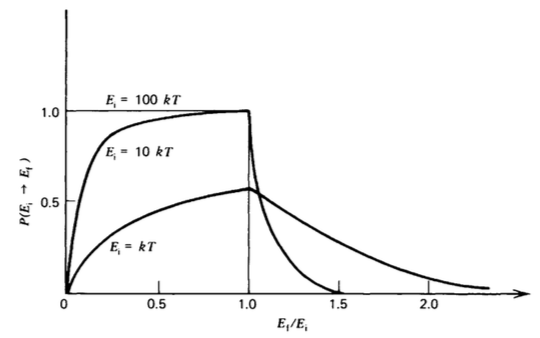
\includegraphics[width=0.5\linewidth]{figures/upscattering.png}
\caption{Differential energy probability distribution as a function relative final energy for three different energies \cite{duderstadt}.}
\label{fig:upscattering}
\end{figure}
